%-----------------------------------------------------------------------------------------------------------------------------------------------%
%	The MIT License (MIT)
%
%	Copyright (c) 2021 Jitin Nair
%
%	Permission is hereby granted, free of charge, to any person obtaining a copy
%	of this software and associated documentation files (the "Software"), to deal
%	in the Software without restriction, including without limitation the rights
%	to use, copy, modify, merge, publish, distribute, sublicense, and/or sell
%	copies of the Software, and to permit persons to whom the Software is
%	furnished to do so, subject to the following conditions:
%	
%	THE SOFTWARE IS PROVIDED "AS IS", WITHOUT WARRANTY OF ANY KIND, EXPRESS OR
%	IMPLIED, INCLUDING BUT NOT LIMITED TO THE WARRANTIES OF MERCHANTABILITY,
%	FITNESS FOR A PARTICULAR PURPOSE AND NONINFRINGEMENT. IN NO EVENT SHALL THE
%	AUTHORS OR COPYRIGHT HOLDERS BE LIABLE FOR ANY CLAIM, DAMAGES OR OTHER
%	LIABILITY, WHETHER IN AN ACTION OF CONTRACT, TORT OR OTHERWISE, ARISING FROM,
%	OUT OF OR IN CONNECTION WITH THE SOFTWARE OR THE USE OR OTHER DEALINGS IN
%	THE SOFTWARE.
%	
%
%-----------------------------------------------------------------------------------------------------------------------------------------------%

%----------------------------------------------------------------------------------------
%	DOCUMENT DEFINITION
%----------------------------------------------------------------------------------------

% article class because we want to fully customize the page and not use a cv template
\documentclass[a4paper,11pt]{article}

%----------------------------------------------------------------------------------------
%	FONT
%----------------------------------------------------------------------------------------

% % fontspec allows you to use TTF/OTF fonts directly
% \usepackage{fontspec}
% \defaultfontfeatures{Ligatures=TeX}

% % modified for ShareLaTeX use
% \setmainfont[
% SmallCapsFont = Fontin-SmallCaps.otf,
% BoldFont = Fontin-Bold.otf,
% ItalicFont = Fontin-Italic.otf
% ]
% {Fontin.otf}

%----------------------------------------------------------------------------------------
%	PACKAGES
%----------------------------------------------------------------------------------------
\usepackage{url}
\usepackage{parskip} 	

%other packages for formatting
\RequirePackage{color}
\RequirePackage{graphicx}
\usepackage[usenames,dvipsnames]{xcolor}
\usepackage[scale=0.92]{geometry}

%tabularx environment
\usepackage{tabularx}

%for lists within experience section
\usepackage{enumitem}
\setlist{itemsep=2pt,topsep=2pt,parsep=0pt,partopsep=0pt}

% centered version of 'X' col. type
\newcolumntype{C}{>{\centering\arraybackslash}X} 

%to prevent spillover of tabular into next pages
\usepackage{supertabular}
\usepackage{tabularx}
\newlength{\fullcollw}
\setlength{\fullcollw}{0.47\textwidth}

%custom \section
\usepackage{titlesec}				
\usepackage{multicol}
\usepackage{multirow}

%CV Sections inspired by: 
%http://stefano.italians.nl/archives/26
\titleformat{\section}{\Large\scshape\raggedright\color{sectioncolor}}{}{0em}{}[\titlerule]
\titlespacing{\section}{0pt}{8pt}{6pt}

%Setup hyperref package, and colours for links
\usepackage[unicode, draft=false]{hyperref}
\definecolor{linkcolour}{rgb}{0,0.2,0.6}
\definecolor{sectioncolor}{rgb}{0,0.2,0.6}
\hypersetup{colorlinks,breaklinks,urlcolor=linkcolour,linkcolor=linkcolour}

%for social icons
\usepackage{fontawesome5}

%debug page outer frames
%\usepackage{showframe}


% job listing environments
\newenvironment{jobshort}[2]
    {
    \begin{tabularx}{\linewidth}{@{}l X r@{}}
    \textbf{#1} & \hfill &  #2 \\[3.75pt]
    \end{tabularx}
    }
    {
    }

\newenvironment{joblong}[2]
    {
    \begin{tabularx}{\linewidth}{@{}l X r@{}}
    \textbf{#1} & \hfill &  #2 \\[3.75pt]
    \end{tabularx}
    \begin{minipage}[t]{\linewidth}
    \begin{itemize}[nosep,after=\strut, leftmargin=1em, itemsep=3pt,label=--]
    }
    {
    \end{itemize}
    \end{minipage}    
    }

%----------------------------------------------------------------------------------------
%	BEGIN DOCUMENT
%----------------------------------------------------------------------------------------
\begin{document}

% non-numbered pages
\pagestyle{empty} 

%----------------------------------------------------------------------------------------
%   TITLE WITH PHOTO (Version Jin)
%----------------------------------------------------------------------------------------

\begin{tabularx}{\linewidth}{@{} X r @{}}
\begin{minipage}[t]{0.72\linewidth}
    \vspace{0.4cm}
    {\Huge{Rahman SUON}} \\[9pt]
    \textbf{INGÉNIEUR DEVOPS \& CLOUD} \\[9pt]
    \href{mailto:contact@rahmansuon.fr}{\faEnvelope\ contact@rahmansuon.fr} \ $|$ \ 
    \href{tel:+33603847905}{\faMobile\ 06 03 84 79 05} \\[3pt]
    \href{https://www.linkedin.com/in/rahman-suon-487a331a4/}{\faLinkedin\ Rahman-Suon} \ $|$ \ 
    \href{https://github.com/Rahman-git7}{\faGithub\ Rahman-git7} \ $|$ \ 
    Paris 
\end{minipage}
&
\begin{minipage}[t]{0.25\linewidth}
    \vspace{0pt}
    \raggedleft
    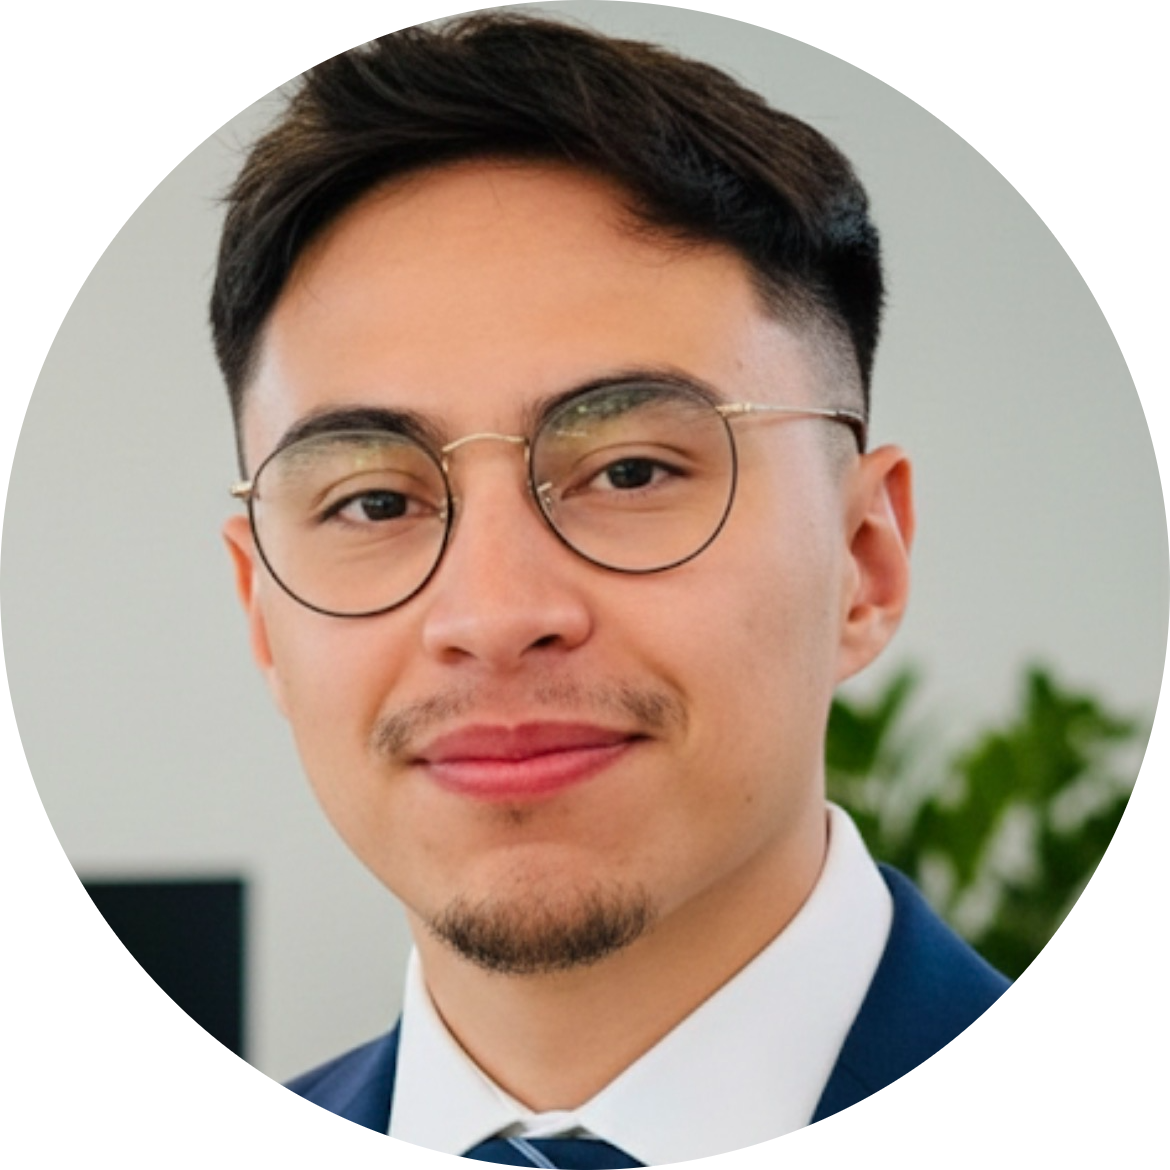
\includegraphics[width=3.2cm,height=3.2cm,keepaspectratio]{photo.png}
\end{minipage}
\\[15pt]
\end{tabularx}

\section{Profil}
Ingénieur DevOps orienté production, j’opère et maintiens des infrastructures cloud AWS en production, avec une pratique des environnements Kubernetes, des chaînes CI/CD, du GitOps et des outils d’observabilité.

\section{Certifications}
\begin{tabularx}{\linewidth}{@{}l X@{}}
{\color{sectioncolor}\raisebox{-0.05\height}\faCloud}\ AWS & 
\href{https://www.credly.com/badges/a6ad431c-313a-42bd-b52f-6158e9cfb49b/public_url}
{\textbf{Certified Solutions Architect – Associate} \textit{(août 2025)}} \\
\end{tabularx}

%----------------------------------------------------------------------------------------
%	EDUCATION
%----------------------------------------------------------------------------------------
\section{Formation}
\begin{tabularx}{\linewidth}{@{}l X@{}}	
2023 - 2025 & Master DevOps \& Cloud - \textbf{SUP DE VINCI}, Paris \\
\end{tabularx}


%----------------------------------------------------------------------------------------
%	SKILLS
%----------------------------------------------------------------------------------------
\section{Stack Technique}
\begin{tabularx}{\linewidth}{@{}l X@{}}
\textbf{Cloud \& Infrastructure} & AWS, Azure, Kubernetes, Docker, Helm, Linux \\[3pt]
\textbf{IaC \& CI/CD} & Terraform, Ansible, Pulumi, GitLab/GitHub Actions, GitOps (ArgoCD) \\[3pt]
\textbf{Monitoring \& Bases de données} & Prometheus, Grafana, ELK Stack, PostgreSQL, Redis \\[3pt]
\textbf{Développement \& Scripting} & Python, Bash, PowerShell, YAML, API REST \\[3pt]
\textbf{Sécurité \& Réseau} & Vault, Secret Manager, SSL/TLS, Load balancing, VPC\\[3pt]
\end{tabularx}

%----------------------------------------------------------------------------------------
% EXPERIENCE SECTIONS
%----------------------------------------------------------------------------------------

%Experience
\section{Expérience Professionnelle}

\begin{joblong}{Ingénieur DevOps Infra Cloud - Efficity, Paris}{2023 - 2025}
\item Exploitation et maintien d’infrastructures cloud AWS en environnements staging et production
\item Déploiement applicatif sur Kubernetes (kubectl, Helm), gestion des Ingress et des configurations associées
\item Mise en œuvre et exploitation d’une approche GitOps avec ArgoCD pour le déploiement continu des applications
\item Interaction avec les pipelines CI/CD existants (GitLab CI) pour assurer la chaîne de déploiement jusqu’aux environnements Kubernetes
\item Conception et déploiement d’une stack d’observabilité complète (Prometheus, Grafana, Loki, Alertmanager, CloudWatch)
\item Supervision proactive des environnements et support aux équipes de développement lors d’incidents ou de phases de débogage
\end{joblong}


\begin{joblong}{Technicien Systèmes et Réseaux - Magnetto Automotive, Aulnay-sous-Bois}{2022 - 2023}
\item Support technique niveau 1-2, gestion Active Directory et maintenance réseau
\item Câblage infrastructure, interventions matérielles et documentation procédures
\end{joblong}

\begin{jobshort}{Technicien Informatique Hotline - Carrefour, Evry}{2021 - 2022}
Diagnostics et résolutions de problèmes relatifs aux ordinateurs de bureaux, portables.
\end{jobshort}

%Projects
\section{Projets Techniques}


\begin{tabularx}{\linewidth}{ @{}l r@{} }
\textbf{Infrastructure DevOps sécurisée} & \hfill \href{https://drive.google.com/file/d/1PlXLjoWP856V7C8GVAYSbwkYGu0XzBrk/view}{Doc} \\[3.75pt]
\multicolumn{2}{@{}X@{}}{Conception et déploiement d’une infrastructure cloud Azure automatisée (Terraform, Ansible), intégrant un cluster Kubernetes (AKS), une chaîne CI/CD et une stack d’observabilité (Grafana), avec des exigences de sécurité et de haute disponibilité.}  \\
\end{tabularx}

\begin{tabularx}{\linewidth}{ @{}l r@{} }
\textbf{API REST sécurisée en Go} & \hfill \href{https://gitlab.com/Rahman-S/api-certificats}{GitLab} \\[3.75pt]
\multicolumn{2}{@{}X@{}}{Développement et mise en production d’une API REST sécurisée en Go (Gin, PocketBase), avec authentification JWT et déploiement automatisé via GitLab CI/CD sur AWS ECS.}  \\
\end{tabularx}



\end{document}